% !TEX spellcheck = en_US



% ~~~~~~~~~~~~~~~~~~~~~~~~~~~~~~~~~~~~~~~ V
% (NC) 2026 Haluk Bingol
% github.com/halukbingol/LaTeX-Templates
%
% Licensees may copy, distribute, display, and perform the work and make derivative works 
% and remixes based on it only for non-commercial purposes. 
% ~~~~~~~~~~~~~~~~~~~~~~~~~~~~~~~~~~~~~~~ A




% v20261123T2200

\documentclass[aspectratio=169,10pt,compress]{beamer}




% ~~~~~~~~~~~~~~~~~~~~~~~~~~~~~~~~~~~~~~~~~~~~~~~~~~~~~~~~~~~~~~~~~ V hblib
	\usepackage{../../hblib/hblibPresentation} % lib presentation: theme, i/N, \hSection, algorithm2e, ...
	\usepackage{../../hblib/hblibCodeoutput} % lib code + output: \lstcode, \lstterminal, ...
	\usepackage{../../hblib/hblibDatastructures} % lib data structures: \hString, \hStack, \hQueue, \hArray, \hGrid
% ~~~~~~~~~~~~~~~~~~~~~~~~~~~~~~~~~~~~~~~~~~~~~~~~~~~~~~~~~~~~~~~~~ A hblib




% +++++++++++++++++++++++++++++++++++++++ V specific
\DontPrintSemicolon % in algorithms
\SetKw{KwAnd}{and}
\SetKw{KwNot}{not}
\SetKw{KwThrow}{throw}
\SetKw{KwGoTo}{continue at}
% +++++++++++++++++++++++++++++++++++++++ A specific



\title[Exceptions, Tests: Concepts]{
	Exception Handling and Unit Testing\\
	Concepts
}
\subtitle{
	\cisOOO\ -- Level 0: ideas and pictures
}
\author[Erkovan]{Sait Erkovan}

\institute[FCIS]{
	Faculty of Computer and Information Sciences\\
	Yeditepe University
}
\date{{\tiny \hbTimeStamp}}

\begin{document}




% ~~~~~~~~~~~~~~~~~~~~~~~~~~~~~~~~~~~~~~ V frm
\begin{frame}[t,fragile]
	\titlepage
\end{frame}
% ~~~~~~~~~~~~~~~~~~~~~~~~~~~~~~~~~~~~~~ A frm




% ~~~~~~~~~~~~~~~~~~~~~~~~~~~~~~~~~~~~~~ V frm
\begin{frame}[t,fragile] \frametitle{Outline}
	\begin{columns}[T]
		\begin{column}{0.48\textwidth}
			\tableofcontents[sections={1-5}, hideallsubsections]
		\end{column}
		\begin{column}{0.48\textwidth}
			\tableofcontents[sections={6-11}, hideallsubsections]
		\end{column}
	\end{columns}

	\vspace{1em}
	\small Ideas only: pictures, tables and pseudo code. Every idea is shown as a Java program in
	\hCode{ExceptionHandling\_UnitTesting-5-examples}.
\end{frame}
% ~~~~~~~~~~~~~~~~~~~~~~~~~~~~~~~~~~~~~~ A frm




% ~~~~~~~~~~~~~~~~~~~~~~~~~~~~~~~~~~~~~~ V
\hSection[Errors]{What can go wrong}
% ~~~~~~~~~~~~~~~~~~~~~~~~~~~~~~~~~~~~~~ A




% ~~~~~~~~~~~~~~~~~~~~~~~~~~~~~~~~~~~~~~ V frm
\begin{frame}[t,fragile] \frametitle{Three kinds of errors}


% +++++++++++++++++++++++++++++++++++++++ V tbl
%: -Tbl. kinds of errors
\begin{table}
		\small
		\begin{tabular}{@{}L{0.15\textwidth}L{0.23\textwidth}L{0.27\textwidth}L{0.26\textwidth}@{}}
			\toprule
			\textbf{Kind} & \textbf{When} & \textbf{Who notices} & \textbf{Example} \\
			\midrule
			compile-time & before the program runs & the compiler, with a message & a missing \hCode{;}, a \hCode{String} into an \hCode{int} \\
			run-time     & while it runs           & the running program: it stops, or an exception is handled & dividing by zero, a missing file \\
			logic        & while it runs           & nobody, unless someone checks the result & an average of 3 instead of 3.5 \\
			\bottomrule
		\end{tabular}
\end{table}%
% +++++++++++++++++++++++++++++++++++++++ A tbl


	\vspace{0.5em}
	\begin{itemize}\small
		\item Compile-time errors are the friendliest: they never reach a user
		\item \hDefined{Exceptions} turn run-time errors into events the program can react to
		\item \hDefined{Tests} are how logic errors are found: they compare results with what is expected
	\end{itemize}
\end{frame}
% ~~~~~~~~~~~~~~~~~~~~~~~~~~~~~~~~~~~~~~ A frm




% ~~~~~~~~~~~~~~~~~~~~~~~~~~~~~~~~~~~~~~ V frm
\begin{frame}[t,fragile] \frametitle{Where problems come from}


% +++++++++++++++++++++++++++++++++++++++ V tbl
%: -Tbl. sources of problems
\begin{table}
		\small
		\begin{tabular}{@{}L{0.16\textwidth}L{0.32\textwidth}L{0.42\textwidth}@{}}
			\toprule
			\textbf{Source} & \textbf{Example} & \textbf{What helps} \\
			\midrule
			the program  & an index one too far; a method called with a wrong value & fix the code; tests find it early \\
			the input    & letters where a number is expected                       & check the input, explain, ask again \\
			the world    & the file is missing, the disk is full, the network is down & report it clearly; maybe try again later \\
			\bottomrule
		\end{tabular}
\end{table}%
% +++++++++++++++++++++++++++++++++++++++ A tbl


	\vspace{0.5em}
	\small The first kind is a \hDefined{bug}. The other two happen even in a correct program, so a correct program
	must be ready for them.
\end{frame}
% ~~~~~~~~~~~~~~~~~~~~~~~~~~~~~~~~~~~~~~ A frm




% ~~~~~~~~~~~~~~~~~~~~~~~~~~~~~~~~~~~~~~ V frm
\begin{frame}[t,fragile] \frametitle{Two paths through a program}
	\begin{center}
		\begin{tikzpicture}[st/.style={draw, rounded corners=2pt, minimum width=2.2cm, minimum height=0.75cm,
				font=\small, fill=white}, ok/.style={-{Latex[length=2mm]}, thick, colorIndex!70!black},
				bad/.style={-{Latex[length=2mm]}, thick, dashed, colorStop}]
			\node[st] (a) at (0,0) {read a value};
			\node[st] (b) at (3.4,0) {compute};
			\node[st] (c) at (6.8,0) {write the result};
			\node[st] (d) at (10.2,0) {next task};
			\node[st, fill=colorHead!50] (h) at (5.1,-2.0) {handler};
			\draw[ok] (a) -- (b);
			\draw[ok] (b) -- (c);
			\draw[ok] (c) -- (d);
			\uncover<2->{\draw[bad] (a.south) |- node[pos=0.25, left, font=\scriptsize] {not a number} (h.west);}
			\uncover<2->{\draw[bad] (b.south) -- node[right, font=\scriptsize, pos=0.4] {divide by 0} (h.north west);}
			\uncover<3->{\draw[ok] (h.east) -| (d.south);}
			\node[font=\scriptsize, colorIndex!70!black] at (5.1,0.65) {the normal path};
			\uncover<2->{\node[font=\scriptsize, colorStop] at (5.1,-2.65) {the exceptional path};}
		\end{tikzpicture}
	\end{center}

	\begin{itemize}\small
		\item Without exceptions, every step needs an \hCode{if} that checks for trouble: the normal path disappears in checks
		\item With exceptions, the normal path is written once; the problems jump to one \hDefined{handler}
		\item<3-> After the handler, the program goes on (or stops in a controlled way)
	\end{itemize}
\end{frame}
% ~~~~~~~~~~~~~~~~~~~~~~~~~~~~~~~~~~~~~~ A frm




% ~~~~~~~~~~~~~~~~~~~~~~~~~~~~~~~~~~~~~~ V
\hSection[Signal]{Signaling a problem}
% ~~~~~~~~~~~~~~~~~~~~~~~~~~~~~~~~~~~~~~ A




% ~~~~~~~~~~~~~~~~~~~~~~~~~~~~~~~~~~~~~~ V frm
\begin{frame}[t,fragile] \frametitle{A special value or an exception?}
	\begin{columns}[T]
		\begin{column}{0.48\textwidth}


% +++++++++++++++++++++++++++++++++++++++ V alg
%: -Alg. find with a special value
\begin{algorithm}[H]
				\caption{Find($a$, $x$): a special value}
				\For{$i \gets 0$ \KwTo $n - 1$}{
				    \If{$a[i] = x$}{\Return $i$\;}
				}
				\Return $-1$ \tcp*{``not found''}
\end{algorithm}
% +++++++++++++++++++++++++++++++++++++++ A alg

		\end{column}
		\begin{column}{0.48\textwidth}


% +++++++++++++++++++++++++++++++++++++++ V alg
%: -Alg. find with an exception
\begin{algorithm}[H]
				\caption{Find($a$, $x$): an exception}
				\For{$i \gets 0$ \KwTo $n - 1$}{
				    \If{$a[i] = x$}{\Return $i$\;}
				}
				\KwThrow NotFound($x$)\;
\end{algorithm}
% +++++++++++++++++++++++++++++++++++++++ A alg

		\end{column}
	\end{columns}


% +++++++++++++++++++++++++++++++++++++++ V tbl
%: -Tbl. special value or exception
\begin{table}
		\footnotesize
		\begin{tabular}{@{}L{0.20\textwidth}L{0.36\textwidth}L{0.36\textwidth}@{}}
			\toprule
			& \textbf{Special value} & \textbf{Exception} \\
			\midrule
			the caller forgets   & $-1$ is used as an index: a crash somewhere else, later & the program stops right here, with a report \\
			every value is valid & no value is left to mean ``error'' (an average can be anything) & no problem: the result and the error are apart \\
			reading the code     & a check after every call                                & the normal path stays short \\
			when it fits         & ``not found'' is normal and expected                     & the method cannot keep its promise \\
			\bottomrule
		\end{tabular}
\end{table}%
% +++++++++++++++++++++++++++++++++++++++ A tbl
\end{frame}
% ~~~~~~~~~~~~~~~~~~~~~~~~~~~~~~~~~~~~~~ A frm




% ~~~~~~~~~~~~~~~~~~~~~~~~~~~~~~~~~~~~~~ V frm
\begin{frame}[t,fragile] \frametitle{Who knows the problem, who knows the fix}
	\begin{center}
		\begin{tikzpicture}[st/.style={draw, rounded corners=2pt, minimum width=3.4cm, minimum height=1.0cm,
				align=center, font=\small, fill=white}]
			\node[st] (ui) at (0,0) {the screen\\ \scriptsize talks to the user};
			\node[st] (svc) at (4.6,0) {the grade book\\ \scriptsize computes averages};
			\node[st, fill=colorUsed!45] (rd) at (9.2,0) {the file reader\\ \scriptsize reads one line};
			\draw[-{Latex[length=2mm]}, thick] (ui) -- node[above, font=\scriptsize] {calls} (svc);
			\draw[-{Latex[length=2mm]}, thick] (svc) -- node[above, font=\scriptsize] {calls} (rd);
			\uncover<2->{\draw[-{Latex[length=2mm]}, thick, dashed, colorStop] (rd.south) to[bend left=25]
				node[below, font=\scriptsize] {line 7 is not a number} (ui.south);}
			\node[font=\scriptsize, align=center] at (9.2,1.0) {knows \emph{what} went wrong};
			\uncover<2->{\node[font=\scriptsize, align=center] at (0,1.0) {knows \emph{what to do}: tell the user};}
		\end{tikzpicture}
	\end{center}

	\vspace{0.5em}
	\begin{itemize}\small
		\item \hDefined{Throw early}: the method that finds the problem reports it at once, with the details
		\item \hDefined{Catch late}: the problem travels up to the first caller that can do something useful
		\item The methods in between need no error code at all
	\end{itemize}
\end{frame}
% ~~~~~~~~~~~~~~~~~~~~~~~~~~~~~~~~~~~~~~ A frm




% ~~~~~~~~~~~~~~~~~~~~~~~~~~~~~~~~~~~~~~ V
\hSection[Stack]{The call stack}
% ~~~~~~~~~~~~~~~~~~~~~~~~~~~~~~~~~~~~~~ A




% ~~~~~~~~~~~~~~~~~~~~~~~~~~~~~~~~~~~~~~ V frm
\begin{frame}[t,fragile] \frametitle{Calls pile up on a stack}
	\begin{columns}[T]
		\begin{column}{0.44\textwidth}
			\begin{center}
				\begin{tikzpicture}[fr/.style={draw, thick, minimum width=3.2cm, minimum height=0.6cm,
						font=\ttfamily\small, fill=white}]
					\node[fr] at (0,0) {main};
					\uncover<2->{\node[fr] at (0,0.65) {report};}
					\uncover<3->{\node[fr] at (0,1.3) {average};}
					\uncover<4->{\node[fr, fill=colorTop!60] at (0,1.95) {readScore};}
					\path (0,2.4);
					\node[font=\scriptsize] at (0,-0.6) {the newest call on top};
				\end{tikzpicture}
			\end{center}
		\end{column}
		\begin{column}{0.54\textwidth}
			\begin{itemize}\small
				\item A call adds a \hDefined{frame} on top: the method's variables and where it is now
				\item A return removes the top frame; its caller goes on
				\item Only the top frame runs; the frames below wait
				\item A run-time report lists these frames, from the top
			\end{itemize}
		\end{column}
	\end{columns}

	\vspace{0.6em}
	\small \hCode{main} calls \hCode{report}, \hCode{report} calls \hCode{average}, \hCode{average} calls \hCode{readScore}.
	Last in, first out: a \hDefined{stack}, the data structure you will build in \hCode{CIS112}.
\end{frame}
% ~~~~~~~~~~~~~~~~~~~~~~~~~~~~~~~~~~~~~~ A frm




% ~~~~~~~~~~~~~~~~~~~~~~~~~~~~~~~~~~~~~~ V frm
\begin{frame}[t,fragile] \frametitle{Unwinding: looking for a handler}
	\begin{columns}[T]
		\begin{column}{0.44\textwidth}
			\begin{center}
				\begin{tikzpicture}[fr/.style={draw, thick, minimum width=3.2cm, minimum height=0.6cm,
						font=\ttfamily\small, fill=white}, note/.style={font=\scriptsize, anchor=west, align=left}]
					\node[fr] at (0,0) {main};
					\only<1-5>{\node[fr] at (0,0.65) {report};}
					\only<5>{\node[fr, fill=colorTop!60] at (0,0.65) {report};
						\node[note] at (1.7,0.65) {has a handler:\\ it runs};}
					\only<1-3>{\node[fr] at (0,1.3) {average};}
					\only<3>{\node[fr, fill=colorUsed!60] at (0,1.3) {average};
						\node[note] at (1.7,1.3) {no handler:\\ removed};}
					\only<1-2>{\node[fr] at (0,1.95) {readScore};}
					\only<1>{\node[fr, fill=colorUsed!60] at (0,1.95) {readScore};
						\node[note] at (1.7,1.95) {throws};}
					\only<2>{\node[fr, fill=colorUsed!60] at (0,1.95) {readScore};
						\node[note] at (1.7,1.95) {no handler:\\ removed};}
					\only<6>{\node[fr, fill=colorTop!60] at (0,0.65) {report};
						\node[note] at (1.7,0.65) {goes on after\\ its handler};}
					\path (0,2.4);
				\end{tikzpicture}
			\end{center}
		\end{column}
		\begin{column}{0.54\textwidth}


% +++++++++++++++++++++++++++++++++++++++ V alg
%: -Alg. find a handler
\begin{algorithm}[H]
				\caption{Unwind($e$)}
				\While{the stack is not empty}{
				    $f \gets$ the top frame\;
				    \If{$f$ is inside a try with a catch for the type of $e$}{
				        run that catch\;
				        \KwGoTo the end of that try in $f$\;
				    }
				    run the finally of $f$, if any\;
				    remove $f$\;
				}
				print the report and stop the program\;
\end{algorithm}
% +++++++++++++++++++++++++++++++++++++++ A alg

		\end{column}
	\end{columns}
\end{frame}
% ~~~~~~~~~~~~~~~~~~~~~~~~~~~~~~~~~~~~~~ A frm




% ~~~~~~~~~~~~~~~~~~~~~~~~~~~~~~~~~~~~~~ V
\hSection[Objects]{Exception objects}
% ~~~~~~~~~~~~~~~~~~~~~~~~~~~~~~~~~~~~~~ A




% ~~~~~~~~~~~~~~~~~~~~~~~~~~~~~~~~~~~~~~ V frm
\begin{frame}[t,fragile] \frametitle{What an exception carries}
	\begin{center}
		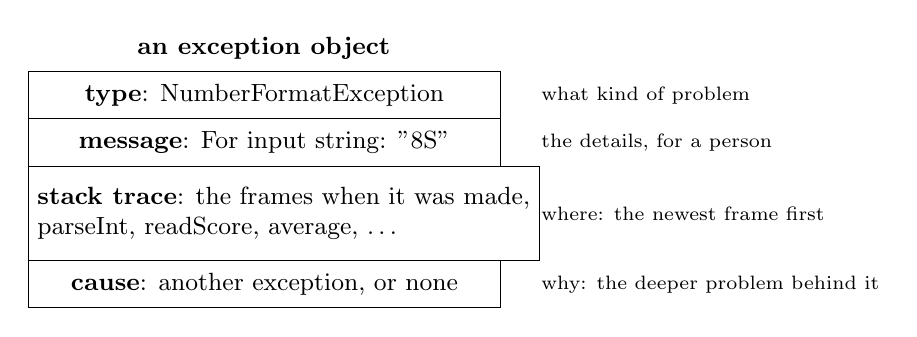
\begin{tikzpicture}[fld/.style={draw, minimum width=6.0cm, minimum height=0.6cm, anchor=west,
				font=\small, fill=white}]
			\node[font=\small\bfseries] at (3.0,0.6) {an exception object};
			\node[fld] (t) at (0,0)     {\textbf{type}: \hCode{NumberFormatException}};
			\node[fld] (m) at (0,-0.6)  {\textbf{message}: \hCode{For input string: "8S"}};
			\node[fld, minimum height=1.2cm, align=left] (s) at (0,-1.5) {\textbf{stack trace}: the frames when it was made,\\
				\hCode{parseInt}, \hCode{readScore}, \hCode{average}, \dots};
			\node[fld] (c) at (0,-2.4)  {\textbf{cause}: another exception, or none};
			\node[font=\scriptsize, anchor=west, align=left] at (6.4,0)     {what kind of problem};
			\node[font=\scriptsize, anchor=west, align=left] at (6.4,-0.6)  {the details, for a person};
			\node[font=\scriptsize, anchor=west, align=left] at (6.4,-1.5)  {where: the newest frame first};
			\node[font=\scriptsize, anchor=west, align=left] at (6.4,-2.4)  {why: the deeper problem behind it};
		\end{tikzpicture}
	\end{center}

	\vspace{0.3em}
	\small An exception is an ordinary object: it is created (\hCode{new}), it can be stored and passed on.
	Throwing it is what makes it special.
\end{frame}
% ~~~~~~~~~~~~~~~~~~~~~~~~~~~~~~~~~~~~~~ A frm




% ~~~~~~~~~~~~~~~~~~~~~~~~~~~~~~~~~~~~~~ V frm
\begin{frame}[t,fragile] \frametitle{Families: a handler catches a whole family}
	\begin{columns}[T]
		\begin{column}{0.50\textwidth}
			\begin{center}
				\begin{tikzpicture}
					\draw[rounded corners=6pt, fill=gray!10] (0,0) rectangle (6.0,4.4);
					\node[font=\scriptsize, anchor=north west] at (0.1,4.35) {all problems};
					\draw[rounded corners=6pt, fill=colorHead!25] (0.3,0.25) rectangle (5.7,3.8);
					\node[font=\scriptsize, anchor=north west] at (0.4,3.75) {problems of the program};
					\draw[rounded corners=6pt, fill=white] (0.6,0.5) rectangle (3.6,3.2);
					\node[font=\scriptsize, anchor=north west] at (0.7,3.15) {a bad argument};
					\draw[rounded corners=6pt, fill=colorTop!30] (0.9,0.75) rectangle (3.3,1.9);
					\node[font=\scriptsize, align=center] at (2.1,1.32) {not a number};
					\draw[rounded corners=6pt, fill=white] (3.8,0.5) rectangle (5.5,3.2);
					\node[font=\scriptsize, align=center] at (4.65,1.85) {a bad\\ index};
				\end{tikzpicture}
			\end{center}
		\end{column}
		\begin{column}{0.48\textwidth}
			\begin{itemize}\small
				\item Exception types form a family tree: a specific type is a kind of a more general one
				\item A handler for a type also catches every type inside it
				\item ``Handle a bad argument'' catches ``not a number'' too
				\item Write specific handlers first: a general one first would take everything
			\end{itemize}
		\end{column}
	\end{columns}

	\vspace{0.4em}
	\small In Java: \hCode{IllegalArgumentException} contains \hCode{NumberFormatException}; both are
	\hCode{RuntimeException}s.
\end{frame}
% ~~~~~~~~~~~~~~~~~~~~~~~~~~~~~~~~~~~~~~ A frm




% ~~~~~~~~~~~~~~~~~~~~~~~~~~~~~~~~~~~~~~ V frm
\begin{frame}[t,fragile] \frametitle{Checked, unchecked, errors}
	\begin{center}
		\begin{tikzpicture}[q/.style={draw, rounded corners=2pt, align=center, font=\small, fill=white, minimum height=0.9cm},
				a/.style={draw, rounded corners=2pt, align=center, font=\small, minimum height=0.9cm},
				ar/.style={-{Latex[length=2mm]}, thick}]
			\node[q] (q1) at (0,0) {Is the Java machine\\ itself in trouble?};
			\node[a, fill=gray!25] (e) at (0,-1.9) {\textbf{error}\\ \scriptsize out of memory: do not catch};
			\node[q] (q2) at (5.0,0) {Can it happen in\\ a correct program?};
			\node[a, fill=colorHead!60] (c) at (5.0,-1.9) {\textbf{checked}\\ \scriptsize a missing file: catch or declare};
			\node[a, fill=white] (u) at (10.0,0) {\textbf{unchecked}\\ \scriptsize a bad index: fix the code};
			\draw[ar] (q1) -- node[left, font=\scriptsize] {yes} (e);
			\draw[ar] (q1) -- node[above, font=\scriptsize] {no} (q2);
			\draw[ar] (q2) -- node[left, font=\scriptsize] {yes} (c);
			\draw[ar] (q2) -- node[above, font=\scriptsize] {no, a bug} (u);
		\end{tikzpicture}
	\end{center}

	\begin{itemize}\small
		\item \hDefined{Checked}: the compiler makes every caller decide: handle it, or say that it passes it on
		\item \hDefined{Unchecked}: allowed to be caught, never required; the real fix is in the code
		\item Java's choice: \hCode{IOException} and its family are checked; \hCode{RuntimeException} and \hCode{Error} are not
	\end{itemize}
\end{frame}
% ~~~~~~~~~~~~~~~~~~~~~~~~~~~~~~~~~~~~~~ A frm




% ~~~~~~~~~~~~~~~~~~~~~~~~~~~~~~~~~~~~~~ V frm
\begin{frame}[t,fragile] \frametitle{Handle or declare}
	\begin{columns}[T]
		\begin{column}{0.50\textwidth}
			\begin{center}
				\begin{tikzpicture}[q/.style={draw, rounded corners=2pt, align=center, font=\small, fill=white},
						ar/.style={-{Latex[length=2mm]}, thick}]
					\node[q] (q) at (0,0) {I call a method that may\\ throw a checked exception};
					\node[q] (f) at (0,-1.5) {Can I do something\\ useful about it here?};
					\node[q, fill=colorTop!40] (h) at (-1.7,-3.1) {\textbf{handle}:\\ try / catch};
					\node[q, fill=colorHead!50] (d) at (1.7,-3.1) {\textbf{declare}:\\ throws in my header};
					\draw[ar] (q) -- (f);
					\draw[ar] (f) -- node[left, font=\scriptsize] {yes} (h);
					\draw[ar] (f) -- node[right, font=\scriptsize] {no} (d);
				\end{tikzpicture}
			\end{center}
		\end{column}
		\begin{column}{0.48\textwidth}
			\begin{itemize}\small
				\item Declaring passes the decision to my caller, who faces the same choice
				\item Declared all the way up through \hCode{main}: the program stops with the report
				\item ``Useful'' means: ask again, use a default, skip the record and count it, tell the user
				\item Printing and going on as if nothing happened is not useful
			\end{itemize}
		\end{column}
	\end{columns}
\end{frame}
% ~~~~~~~~~~~~~~~~~~~~~~~~~~~~~~~~~~~~~~ A frm




% ~~~~~~~~~~~~~~~~~~~~~~~~~~~~~~~~~~~~~~ V
\hSection[Cleanup]{Cleaning up}
% ~~~~~~~~~~~~~~~~~~~~~~~~~~~~~~~~~~~~~~ A




% ~~~~~~~~~~~~~~~~~~~~~~~~~~~~~~~~~~~~~~ V frm
\begin{frame}[t,fragile] \frametitle{finally: on every path}
	\begin{center}
		\begin{tikzpicture}[b/.style={draw, rounded corners=2pt, minimum height=0.55cm, font=\scriptsize, fill=white},
				ar/.style={-{Latex[length=1.6mm]}, thick}]
			\foreach \y/\t in {0/{no exception}, -1.1/{an exception, caught}, -2.2/{an exception, not caught}}
				\node[font=\small, anchor=east] at (-0.2,\y) {\t};
			% path 1
			\node[b, minimum width=2.4cm] (t1) at (1.3,0) {try: all of it};
			\node[b, minimum width=1.6cm, fill=colorHead!50] (f1) at (4.6,0) {finally};
			\node[b, minimum width=2.4cm] (n1) at (7.6,0) {next statement};
			\draw[ar] (t1) -- (f1); \draw[ar] (f1) -- (n1);
			% path 2
			\node[b, minimum width=1.2cm] (t2) at (0.7,-1.1) {try: part};
			\node[b, minimum width=1.2cm, fill=colorTop!40] (c2) at (2.3,-1.1) {catch};
			\node[b, minimum width=1.6cm, fill=colorHead!50] (f2) at (4.6,-1.1) {finally};
			\node[b, minimum width=2.4cm] (n2) at (7.6,-1.1) {next statement};
			\draw[ar] (t2) -- (c2); \draw[ar] (c2) -- (f2); \draw[ar] (f2) -- (n2);
			% path 3
			\node[b, minimum width=1.2cm] (t3) at (0.7,-2.2) {try: part};
			\node[b, minimum width=1.6cm, fill=colorHead!50] (f3) at (4.6,-2.2) {finally};
			\node[b, minimum width=2.4cm, fill=colorUsed!50] (n3) at (7.6,-2.2) {to the caller};
			\draw[ar] (t3) -- (f3); \draw[ar] (f3) -- (n3);
		\end{tikzpicture}
	\end{center}

	\vspace{0.3em}
	\begin{itemize}\small
		\item Whatever happens in the \hCode{try}, the \hCode{finally} part runs before the program leaves the block
		\item It is the place for work that must always be done: close a file, give back what was borrowed
		\item It runs even when the \hCode{try} returns
	\end{itemize}
\end{frame}
% ~~~~~~~~~~~~~~~~~~~~~~~~~~~~~~~~~~~~~~ A frm




% ~~~~~~~~~~~~~~~~~~~~~~~~~~~~~~~~~~~~~~ V frm
\begin{frame}[t,fragile] \frametitle{Resources: open, use, close}
	\begin{center}
		\begin{tikzpicture}[b/.style={draw, rounded corners=2pt, minimum height=0.6cm, minimum width=1.9cm,
				font=\scriptsize, fill=white}, ar/.style={-{Latex[length=1.6mm]}, thick}]
			\node[b, fill=colorTop!40] (oa) at (0,0) {open input};
			\node[b, fill=colorTop!40] (ob) at (2.4,0) {open output};
			\node[b] (u) at (4.8,0) {use both};
			\node[b, fill=colorHead!50] (cb) at (7.2,0) {close output};
			\node[b, fill=colorHead!50] (ca) at (9.6,0) {close input};
			\draw[ar] (oa) -- (ob); \draw[ar] (ob) -- (u); \draw[ar] (u) -- (cb); \draw[ar] (cb) -- (ca);
			\draw[decorate, decoration={brace, amplitude=5pt, mirror}] (-0.9,-0.45) -- (10.5,-0.45)
				node[midway, below=6pt, font=\scriptsize] {a try-with-resources block: the closing is automatic};
		\end{tikzpicture}
	\end{center}

	\begin{itemize}\small
		\item A \hDefined{resource} is something borrowed from the system: an open file, a network connection
		\item There are only so many; an open file may also hold data that is not written yet
		\item \hCode{try (open A; open B) \{ use \}} closes them for you, in reverse order, with or without an exception
		\item If closing fails too, the first problem is kept and the closing problem is attached to it
	\end{itemize}
\end{frame}
% ~~~~~~~~~~~~~~~~~~~~~~~~~~~~~~~~~~~~~~ A frm




% ~~~~~~~~~~~~~~~~~~~~~~~~~~~~~~~~~~~~~~ V
\hSection[Design]{Designing with exceptions}
% ~~~~~~~~~~~~~~~~~~~~~~~~~~~~~~~~~~~~~~ A




% ~~~~~~~~~~~~~~~~~~~~~~~~~~~~~~~~~~~~~~ V frm
\begin{frame}[t,fragile] \frametitle{A method is a contract}
	\begin{center}
		\begin{tikzpicture}[ar/.style={-{Latex[length=2mm]}, thick}]
			\node[draw, rounded corners=3pt, minimum width=3.6cm, minimum height=1.3cm, align=center, font=\small,
				fill=colorHead!30] (m) at (0,0) {\hCode{letterGrade(score)}};
			\node[align=center, font=\scriptsize] (pre) at (-4.6,0) {\textbf{precondition}\\ the caller promises:\\ $0 \le score \le 100$};
			\node[align=center, font=\scriptsize] (post) at (4.6,0) {\textbf{postcondition}\\ the method promises:\\ the right letter, A to F};
			\draw[ar] (pre) -- (m); \draw[ar] (m) -- (post);
			\node[align=center, font=\scriptsize, colorStop] at (0,-1.3) {precondition broken: the method throws at once};
		\end{tikzpicture}
	\end{center}

	\begin{itemize}\small
		\item The \hDefined{precondition} is what the method needs; the \hDefined{postcondition} is what it gives back
		\item \hDefined{Fail fast}: check the precondition first. A bad value stored and used later fails far from its cause
		\item Write the contract down (in the comment above the method); tests check the postcondition
	\end{itemize}
\end{frame}
% ~~~~~~~~~~~~~~~~~~~~~~~~~~~~~~~~~~~~~~ A frm




% ~~~~~~~~~~~~~~~~~~~~~~~~~~~~~~~~~~~~~~ V frm
\begin{frame}[t,fragile] \frametitle{Patterns and anti-patterns}


% +++++++++++++++++++++++++++++++++++++++ V tbl
%: -Tbl. patterns and anti-patterns
\begin{table}
		\footnotesize
		\begin{tabular}{@{}L{0.24\textwidth}L{0.36\textwidth}L{0.32\textwidth}@{}}
			\toprule
			\textbf{Anti-pattern} & \textbf{What goes wrong} & \textbf{Instead} \\
			\midrule
			swallowing: an empty handler     & the problem disappears; wrong results later & handle it, or let it go up \\
			catch-all for everything          & hides bugs together with the expected problems & catch the specific types \\
			a vague message: ``error''        & nobody can tell what or where               & say what, with the value \\
			exceptions instead of a check     & slow and hard to read                      & check with \hCode{if} when you can \\
			report and go on                  & the next step works with garbage            & stop that task, or repair the data \\
			the same problem reported twice   & two reports, one problem                    & report it once, where it is handled \\
			\bottomrule
		\end{tabular}
\end{table}%
% +++++++++++++++++++++++++++++++++++++++ A tbl
\end{frame}
% ~~~~~~~~~~~~~~~~~~~~~~~~~~~~~~~~~~~~~~ A frm




% ~~~~~~~~~~~~~~~~~~~~~~~~~~~~~~~~~~~~~~ V
\hSection[Why test]{Why test}
% ~~~~~~~~~~~~~~~~~~~~~~~~~~~~~~~~~~~~~~ A




% ~~~~~~~~~~~~~~~~~~~~~~~~~~~~~~~~~~~~~~ V frm
\begin{frame}[t,fragile] \frametitle{Testing and debugging}


% +++++++++++++++++++++++++++++++++++++++ V tbl
%: -Tbl. testing and debugging
\begin{table}
		\small
		\begin{tabular}{@{}L{0.18\textwidth}L{0.36\textwidth}L{0.36\textwidth}@{}}
			\toprule
			& \textbf{Testing} & \textbf{Debugging} \\
			\midrule
			question   & \emph{is} something wrong?                      & \emph{where} and \emph{why} is it wrong? \\
			starts     & with what the program should do               & with a failure: a red test, a report \\
			result     & pass or fail, for chosen inputs               & the faulty line, then a fix \\
			repeated   & automatically, after every change             & by hand, once per bug \\
			\bottomrule
		\end{tabular}
\end{table}%
% +++++++++++++++++++++++++++++++++++++++ A tbl


	\vspace{0.6em}
	\begin{center}
		\begin{tikzpicture}[b/.style={draw, rounded corners=2pt, minimum height=0.7cm, minimum width=2.2cm,
				font=\small, fill=white}, ar/.style={-{Latex[length=2mm]}, thick}]
			\node[b] (w) at (0,0) {write code};
			\node[b] (t) at (3.2,0) {run tests};
			\node[b, fill=colorUsed!40] (d) at (6.4,0) {debug};
			\node[b, fill=colorTop!40] (g) at (9.6,0) {green: done};
			\draw[ar] (w) -- (t); \draw[ar] (t) -- node[above, font=\scriptsize] {red} (d);
			\draw[ar] (d.south) to[bend left=30] node[below, font=\scriptsize] {fix} (t.south);
			\draw[ar] (t.north) to[bend left=30] node[above, font=\scriptsize] {green} (g.north);
		\end{tikzpicture}
	\end{center}
\end{frame}
% ~~~~~~~~~~~~~~~~~~~~~~~~~~~~~~~~~~~~~~ A frm




% ~~~~~~~~~~~~~~~~~~~~~~~~~~~~~~~~~~~~~~ V frm
\begin{frame}[t,fragile] \frametitle{The later a bug is found, the more it costs}
	\begin{center}
		\begin{tikzpicture}
			\foreach \x/\h/\t in {0/0.4/{while\\ writing}, 2.3/0.8/{by a\\ unit test}, 4.6/1.5/{by a\\ classmate}, 6.9/2.4/{at the\\ exam}, 9.2/3.4/{by a\\ user}} {
				\fill[colorUsed!60] (\x,0) rectangle (\x+1.3,\h);
				\node[font=\scriptsize, align=center, below] at (\x+0.65,0) {\t};
			}
			\draw[thick] (-0.3,0) -- (10.8,0);
			\draw[-{Latex[length=2mm]}, thick] (-0.3,0) -- (-0.3,3.8) node[above, font=\scriptsize] {cost};
		\end{tikzpicture}
	\end{center}

	\small A picture of the idea, not measured numbers. Found late, a bug costs more time to locate
	(the code is no longer fresh in mind), more work to fix (more code depends on it), and sometimes trust or grades.
	Unit tests find bugs at the second bar.
\end{frame}
% ~~~~~~~~~~~~~~~~~~~~~~~~~~~~~~~~~~~~~~ A frm




% ~~~~~~~~~~~~~~~~~~~~~~~~~~~~~~~~~~~~~~ V frm
\begin{frame}[t,fragile] \frametitle{Kinds of tests}
	\begin{columns}[T]
		\begin{column}{0.46\textwidth}
			\begin{center}
				\begin{tikzpicture}
					\fill[colorTop!40] (0,0) -- (5.0,0) -- (4.1,1.2) -- (0.9,1.2) -- cycle;
					\fill[colorHead!50] (0.9,1.2) -- (4.1,1.2) -- (3.2,2.4) -- (1.8,2.4) -- cycle;
					\fill[colorUsed!45] (1.8,2.4) -- (3.2,2.4) -- (2.5,3.4) -- cycle;
					\node[font=\small] at (2.5,0.6) {unit tests: many};
					\node[font=\small] at (2.5,1.8) {integration};
					\node[font=\scriptsize] at (2.5,2.75) {system};
				\end{tikzpicture}
			\end{center}
		\end{column}
		\begin{column}{0.52\textwidth}
			\begin{itemize}\small
				\item \hDefined{Unit test}: one method or class, alone; fast, many of them
				\item \hDefined{Integration test}: parts together, e.g. reading a real file
				\item \hDefined{System test}: the whole program, as a user uses it; slow, few
				\item Higher in the pyramid: closer to the user, slower, harder to locate a bug
			\end{itemize}
		\end{column}
	\end{columns}

	\vspace{0.4em}
	\small This topic is about the bottom layer: \hDefined{unit tests}.
\end{frame}
% ~~~~~~~~~~~~~~~~~~~~~~~~~~~~~~~~~~~~~~ A frm




% ~~~~~~~~~~~~~~~~~~~~~~~~~~~~~~~~~~~~~~ V
\hSection[Unit]{Unit tests}
% ~~~~~~~~~~~~~~~~~~~~~~~~~~~~~~~~~~~~~~ A




% ~~~~~~~~~~~~~~~~~~~~~~~~~~~~~~~~~~~~~~ V frm
\begin{frame}[t,fragile] \frametitle{Anatomy of a test case}
	\begin{center}
		\begin{tikzpicture}[b/.style={draw, rounded corners=2pt, minimum height=0.8cm, align=center, font=\small, fill=white},
				ar/.style={-{Latex[length=2mm]}, thick}]
			\node[b, fill=colorTop!30, minimum width=2.6cm] (a) at (0,0) {\textbf{arrange}\\ \scriptsize score = 85};
			\node[b, fill=colorHead!40, minimum width=2.6cm] (b) at (3.6,0) {\textbf{act}\\ \scriptsize actual = letterGrade(85)};
			\node[b, fill=colorUsed!35, minimum width=2.6cm] (c) at (7.6,0) {\textbf{assert}\\ \scriptsize actual = expected?};
			\node[b, minimum width=2.0cm] (o) at (7.6,1.6) {\textbf{oracle}\\ \scriptsize expected = B};
			\node[b, minimum width=1.4cm] (r) at (10.6,0) {pass\\ or fail};
			\draw[ar] (a) -- (b); \draw[ar] (b) -- (c); \draw[ar] (o) -- (c); \draw[ar] (c) -- (r);
		\end{tikzpicture}
	\end{center}

	\begin{itemize}\small
		\item \hDefined{Arrange} the input, \hDefined{act} (call the unit once), \hDefined{assert} (compare with the expected value)
		\item The \hDefined{oracle} gives the expected value: worked out by hand, a table, a slower but simple method,
			  or a property (``the result is sorted'')
		\item A \hDefined{test suite} is a set of test cases; it can be run at any time, again and again
	\end{itemize}
\end{frame}
% ~~~~~~~~~~~~~~~~~~~~~~~~~~~~~~~~~~~~~~ A frm




% ~~~~~~~~~~~~~~~~~~~~~~~~~~~~~~~~~~~~~~ V frm
\begin{frame}[t,fragile] \frametitle{A test runner}
	\begin{columns}[T]
		\begin{column}{0.54\textwidth}


% +++++++++++++++++++++++++++++++++++++++ V alg
%: -Alg. run all tests
\begin{algorithm}[H]
				\caption{RunAll($tests$)}
				$pass \gets 0$; $fail \gets 0$; $error \gets 0$\;
				\ForEach{test $t$ in $tests$}{
				    run $t$ in a new, clean setting\;
				    \uIf{an assertion of $t$ was false}{$fail \gets fail + 1$\;}
				    \uElseIf{$t$ threw another exception}{$error \gets error + 1$\;}
				    \Else{$pass \gets pass + 1$\;}
				}
				report $pass$, $fail$, $error$\;
\end{algorithm}
% +++++++++++++++++++++++++++++++++++++++ A alg

		\end{column}
		\begin{column}{0.44\textwidth}


% +++++++++++++++++++++++++++++++++++++++ V tbl
%: -Tbl. three outcomes
\begin{table}
				\footnotesize
				\begin{tabular}{@{}L{0.24\textwidth}L{0.68\textwidth}@{}}
					\toprule
					\textbf{Outcome} & \textbf{Means} \\
					\midrule
					pass    & every assertion held \\
					failure & an assertion was false: a wrong result \\
					error   & an unexpected exception: it crashed \\
					\bottomrule
				\end{tabular}
\end{table}%
% +++++++++++++++++++++++++++++++++++++++ A tbl


			\small A failing assertion is itself an exception: the runner tells the two apart by type.
			One test does not stop the others.
		\end{column}
	\end{columns}
\end{frame}
% ~~~~~~~~~~~~~~~~~~~~~~~~~~~~~~~~~~~~~~ A frm




% ~~~~~~~~~~~~~~~~~~~~~~~~~~~~~~~~~~~~~~ V frm
\begin{frame}[t,fragile] \frametitle{Good tests}


% +++++++++++++++++++++++++++++++++++++++ V tbl
%: -Tbl. properties of a good test
\begin{table}
		\small
		\begin{tabular}{@{}L{0.20\textwidth}L{0.72\textwidth}@{}}
			\toprule
			\textbf{Property} & \textbf{Means} \\
			\midrule
			automatic    & it decides pass or fail by itself; nobody reads printed output \\
			repeatable   & the same result every time: no random input, no clock, no order between tests \\
			independent  & it does not need another test to run first \\
			focused      & one idea per test; its name says which \\
			fast         & hundreds run in seconds, so they are run often \\
			honest       & the expected value comes from the oracle, never from the code under test \\
			\bottomrule
		\end{tabular}
\end{table}%
% +++++++++++++++++++++++++++++++++++++++ A tbl
\end{frame}
% ~~~~~~~~~~~~~~~~~~~~~~~~~~~~~~~~~~~~~~ A frm




% ~~~~~~~~~~~~~~~~~~~~~~~~~~~~~~~~~~~~~~ V
\hSection[Choose]{Choosing test cases}
% ~~~~~~~~~~~~~~~~~~~~~~~~~~~~~~~~~~~~~~ A




% ~~~~~~~~~~~~~~~~~~~~~~~~~~~~~~~~~~~~~~ V frm
\begin{frame}[t,fragile] \frametitle{Classes and boundaries}
	\begin{center}
		\begin{tikzpicture}[x=0.78cm]
			\fill[gray!25]     (-1.5,0) rectangle (0,0.6);
			\fill[colorTop!30]  (0,0)   rectangle (7,0.6);
			\fill[colorHead!40] (7,0)   rectangle (12,0.6);
			\fill[colorUsed!35] (12,0)  rectangle (15,0.6);
			\node[font=\scriptsize] at (-0.75,0.3) {illegal};
			\node[font=\scriptsize] at (3.5,0.3)   {free: age 0 to 6};
			\node[font=\scriptsize] at (9.5,0.3)   {child: 7 to 17};
			\node[font=\scriptsize] at (13.5,0.3)  {adult: 18 and up};
			\foreach \x/\l in {0/{-1 | 0}, 7/{6 | 7}, 12/{17 | 18}}
				\node[font=\ttfamily\scriptsize, colorStop, below] at (\x,0) {\l};
			\foreach \x in {3.5, 9.5, 13.5}
				\fill[colorIndex] (\x,0.85) circle (0.07);
			\node[font=\scriptsize, colorIndex, anchor=east] at (3.2,0.85) {one per class};
		\end{tikzpicture}
	\end{center}

	\begin{itemize}\small
		\item An \hDefined{equivalence class} is a set of inputs the method treats alike: one test from each is enough
		\item A \hDefined{boundary} is where the behavior changes: test both sides; most mistakes are there (\hCode{<} or \hCode{<=}?)
		\item Do not forget the illegal class: what must happen there? (an exception)
		\item For a ticket price by age: about 3 + 6 + 1 tests instead of hundreds of ages
	\end{itemize}
\end{frame}
% ~~~~~~~~~~~~~~~~~~~~~~~~~~~~~~~~~~~~~~ A frm




% ~~~~~~~~~~~~~~~~~~~~~~~~~~~~~~~~~~~~~~ V frm
\begin{frame}[t,fragile] \frametitle{Special values}


% +++++++++++++++++++++++++++++++++++++++ V tbl
%: -Tbl. special values
\begin{table}
		\small
		\begin{tabular}{@{}L{0.16\textwidth}L{0.76\textwidth}@{}}
			\toprule
			\textbf{Input} & \textbf{Try} \\
			\midrule
			a number  & 0, 1, $-1$, the largest and the smallest (\hCode{Integer.MAX\_VALUE}), an exact boundary \\
			an array  & empty, one element, all equal, all negative, the answer first or last, sorted, reversed \\
			a string  & empty, one character, only spaces, upper and lower case, Turkish letters (İ, ı) \\
			a file    & missing, empty, one line, a line that is not a number, no newline at the end \\
			a table   & no rows, one row, rows of different lengths \\
			\bottomrule
		\end{tabular}
\end{table}%
% +++++++++++++++++++++++++++++++++++++++ A tbl


	\vspace{0.5em}
	\small A classic: the largest element of an array, with the start value 0. All tests pass until one array
	is all negative.
\end{frame}
% ~~~~~~~~~~~~~~~~~~~~~~~~~~~~~~~~~~~~~~ A frm




% ~~~~~~~~~~~~~~~~~~~~~~~~~~~~~~~~~~~~~~ V frm
\begin{frame}[t,fragile] \frametitle{Black box, white box, coverage}
	\begin{columns}[T]
		\begin{column}{0.44\textwidth}
			\begin{center}
				\begin{tikzpicture}[b/.style={draw, rounded corners=2pt, align=center, font=\scriptsize, fill=white,
						minimum width=1.9cm, minimum height=0.6cm}, d/.style={draw, rounded corners=6pt, font=\scriptsize,
						inner sep=3pt, fill=white}, ar/.style={-{Latex[length=1.6mm]}, thick}]
					\node[d] (q) at (0,0) {express?};
					\node[b, fill=colorTop!35] (y) at (-1.6,-1.3) {cost $\times$ 2};
					\only<1>{\node[b] (n) at (1.6,-1.3) {cost + 5};}
					\only<2->{\node[b, fill=colorTop!35] (n) at (1.6,-1.3) {cost + 5};}
					\node[b, fill=colorTop!35] (r) at (0,-2.6) {return cost};
					\draw[ar] (q) -| node[pos=0.2, above, font=\scriptsize] {yes} (y);
					\draw[ar] (q) -| node[pos=0.2, above, font=\scriptsize] {no} (n);
					\draw[ar] (y) |- (r); \draw[ar] (n) |- (r);
				\end{tikzpicture}

				\scriptsize \only<1>{tests so far: only express orders}\only<2->{one more test: a normal order}
			\end{center}
		\end{column}
		\begin{column}{0.54\textwidth}
			\begin{itemize}\small
				\item \hDefined{Black box}: tests from the description only (classes, boundaries)
				\item \hDefined{White box}: tests that look at the code too, e.g. every branch
				\item \hDefined{Coverage}: the part of the code that the tests run. A line no test runs may hide any bug
				\item<2-> 100\% coverage is not ``no bugs'': a line can run and still compute the wrong value
			\end{itemize}
		\end{column}
	\end{columns}
\end{frame}
% ~~~~~~~~~~~~~~~~~~~~~~~~~~~~~~~~~~~~~~ A frm




% ~~~~~~~~~~~~~~~~~~~~~~~~~~~~~~~~~~~~~~ V
\hSection[Time]{Tests over time}
% ~~~~~~~~~~~~~~~~~~~~~~~~~~~~~~~~~~~~~~ A




% ~~~~~~~~~~~~~~~~~~~~~~~~~~~~~~~~~~~~~~ V frm
\begin{frame}[t,fragile] \frametitle{Regression: a bug fixed stays fixed}
	\begin{center}
		\begin{tikzpicture}[b/.style={draw, rounded corners=2pt, align=center, font=\scriptsize, fill=white,
				minimum height=0.9cm, text width=2.0cm}, ar/.style={-{Latex[length=2mm]}, thick}]
			\node[b, fill=colorUsed!40] (r) at (0,0) {a bug report:\\ 100 gives an error};
			\node[b, fill=colorUsed!20] (t) at (2.9,0) {a new test for 100: red};
			\node[b] (f) at (5.8,0) {fix the code};
			\node[b, fill=colorTop!35] (g) at (8.7,0) {all tests green};
			\node[b, fill=colorTop!20] (k) at (11.6,0) {the test stays, run after every change};
			\draw[ar] (r) -- (t); \draw[ar] (t) -- (f); \draw[ar] (f) -- (g); \draw[ar] (g) -- (k);
		\end{tikzpicture}
	\end{center}

	\begin{itemize}\small
		\item A \hDefined{regression} is a bug that comes back, or a working feature that breaks after a change
		\item Write the test \emph{before} the fix: it must be red first, so you know it can see the bug
		\item The suite grows with every bug: it remembers what went wrong before
	\end{itemize}
\end{frame}
% ~~~~~~~~~~~~~~~~~~~~~~~~~~~~~~~~~~~~~~ A frm




% ~~~~~~~~~~~~~~~~~~~~~~~~~~~~~~~~~~~~~~ V frm
\begin{frame}[t,fragile] \frametitle{Test first: red, green, refactor}
	\begin{columns}[T]
		\begin{column}{0.44\textwidth}
			\begin{center}
				\begin{tikzpicture}[c/.style={circle, draw, thick, minimum size=1.6cm, align=center, font=\small},
						ar/.style={-{Latex[length=2mm]}, thick}]
					\node[c, fill=colorUsed!55] (r) at (90:1.6) {red};
					\node[c, fill=colorTop!50] (g) at (330:1.6) {green};
					\node[c, fill=colorIndex!30] (f) at (210:1.6) {refactor};
					\draw[ar] (r) to[bend left=25] (g);
					\draw[ar] (g) to[bend left=25] (f);
					\draw[ar] (f) to[bend left=25] (r);
				\end{tikzpicture}
			\end{center}
		\end{column}
		\begin{column}{0.54\textwidth}
			\begin{enumerate}\small
				\item \textbf{Red}: write one small test for behavior that does not exist yet; it fails
				\item \textbf{Green}: write the simplest code that makes it pass
				\item \textbf{Refactor}: make the code clean; the tests must stay green
				\item Repeat with the next small test
			\end{enumerate}

			\vspace{0.5em}
			\small Called \hDefined{test-driven development}. The tests are a precise description of what to build,
			written before the building starts.
		\end{column}
	\end{columns}
\end{frame}
% ~~~~~~~~~~~~~~~~~~~~~~~~~~~~~~~~~~~~~~ A frm




% ~~~~~~~~~~~~~~~~~~~~~~~~~~~~~~~~~~~~~~ V frm
\begin{frame}[t,fragile] \frametitle{What tests can and cannot show}
	\begin{columns}[T]
		\begin{column}{0.44\textwidth}
			\begin{center}
				\begin{tikzpicture}
					\draw[rounded corners=6pt, fill=gray!8] (0,0) rectangle (5.2,3.4);
					\node[font=\scriptsize, anchor=north west] at (0.1,3.35) {all possible inputs};
					\foreach \x/\y in {0.6/0.6, 1.4/2.1, 2.2/1.2, 3.1/2.6, 3.8/0.9, 4.5/1.9}
						\fill[colorTop!80!black] (\x,\y) circle (0.09);
					\foreach \x/\y in {1.0/1.5, 2.8/0.5, 4.2/2.8}
						\fill[colorIndex] (\x,\y) circle (0.09);
					\fill[colorStop] (3.4,1.6) circle (0.09);
					\node[font=\scriptsize, colorStop, anchor=west] at (3.5,1.6) {a bug};
				\end{tikzpicture}

				\scriptsize green: visible tests; blue: hidden tests
			\end{center}
		\end{column}
		\begin{column}{0.54\textwidth}
			\begin{itemize}\small
				\item Tests try a few points of a huge input space
				\item A red test proves there is a bug; all green proves only that these points work
				\item Code written just to pass the visible tests often fails the hidden ones: the course grader
					  uses both kinds
				\item Good choice of points (classes, boundaries, special values) makes green mean much more
			\end{itemize}
		\end{column}
	\end{columns}
\end{frame}
% ~~~~~~~~~~~~~~~~~~~~~~~~~~~~~~~~~~~~~~ A frm




% ~~~~~~~~~~~~~~~~~~~~~~~~~~~~~~~~~~~~~~ V
\hSection[End]{Summary}
% ~~~~~~~~~~~~~~~~~~~~~~~~~~~~~~~~~~~~~~ A




% ~~~~~~~~~~~~~~~~~~~~~~~~~~~~~~~~~~~~~~ V frm
\begin{frame}[t,fragile] \frametitle{Glossary}


% +++++++++++++++++++++++++++++++++++++++ V tbl
%: -Tbl. glossary
\begin{table}
		\scriptsize
		\begin{tabular}{@{}L{0.15\textwidth}L{0.30\textwidth}L{0.17\textwidth}L{0.29\textwidth}@{}}
			\toprule
			\textbf{Term} & \textbf{Meaning} & \textbf{Term} & \textbf{Meaning} \\
			\midrule
			exception   & an object that reports a run-time problem   & unit test     & checks one method or class alone \\
			throw       & report it; the method ends at once          & assertion     & a comparison with the expected value \\
			handler     & code that reacts to it (catch)              & oracle        & where the expected value comes from \\
			call stack  & the methods called and not yet returned     & failure / error & a false assertion / an unexpected exception \\
			unwinding   & removing frames until a handler             & equivalence class & inputs treated alike \\
			checked     & the compiler makes you handle or declare it & boundary      & where the behavior changes \\
			unchecked   & a bug or a bad value; no rule               & coverage      & the code that the tests run \\
			finally     & runs on every path                          & regression    & a fixed bug that comes back \\
			resource    & borrowed from the system; must be closed    & test first    & red, green, refactor \\
			contract    & precondition and postcondition              & test suite    & all tests, run at any time \\
			\bottomrule
		\end{tabular}
\end{table}%
% +++++++++++++++++++++++++++++++++++++++ A tbl
\end{frame}
% ~~~~~~~~~~~~~~~~~~~~~~~~~~~~~~~~~~~~~~ A frm




% ~~~~~~~~~~~~~~~~~~~~~~~~~~~~~~~~~~~~~~ V frm
\begin{frame}[t,fragile] \frametitle{Exercises (paper and pencil)}
	\begin{enumerate}\small
		\item For each, say: a bug, bad input or the world? Checked or unchecked? \\
			  a missing file; $-1$ as an index; ``twelve'' typed for a number; the disk is full
		\item Draw the call stack of \hCode{main} $\to$ \hCode{a} $\to$ \hCode{b} $\to$ \hCode{c}; \hCode{c} throws, \hCode{a} handles.
			  Which frames are removed, in which order?
		\item A method returns $-1$ for ``not found''. Give an input where this is safe, and one where it is not
		\item Write the contract of \hCode{average(scores)}. What should happen for an empty array?
		\item Equivalence classes and boundaries for: a password must have 8 to 20 characters
		\item List the special values you would test for ``the second largest element of an array''
		\item Red, green, refactor: describe the first three tests for ``seconds to hh:mm:ss''
	\end{enumerate}
\end{frame}
% ~~~~~~~~~~~~~~~~~~~~~~~~~~~~~~~~~~~~~~ A frm




% ~~~~~~~~~~~~~~~~~~~~~~~~~~~~~~~~~~~~~~ V frm
\begin{frame}[t,fragile] \frametitle{Where to go next}
	\begin{itemize}\small
		\item \hCode{ExceptionHandling\_UnitTesting-5-examples}: every idea of this deck as a small Java program
		\item \hCode{-1-freshman}: the messages, the common mistakes, the first JUnit tests
		\item \hCode{-2-sophomore}: designing with exceptions, your own exception types, JUnit in depth
		\item \hCode{-3-junior}: the cost of exceptions, test doubles, measuring the quality of tests
		\item \hCode{-4-senior}: exceptions inside the JVM, security, production, how JUnit works
	\end{itemize}
\end{frame}
% ~~~~~~~~~~~~~~~~~~~~~~~~~~~~~~~~~~~~~~ A frm




% ~~~~~~~~~~~~~~~~~~~~~~~~~~~~~~~~~~~~~~ V frm
\begin{frame}[t,fragile] \frametitle{References}
	\small The Java Tutorials, lesson Exceptions \cite{TheJavaTutorials}; JUnit \cite{homeJunit}; Big Java \cite{horstmann2016big}.

	\vspace{1em}
	\setbeamertemplate{bibliography item}[text]
	\bibliographystyle{IEEEtran}
	\tiny\bibliography{../../hblib/hblibDataStructures}
\end{frame}
% ~~~~~~~~~~~~~~~~~~~~~~~~~~~~~~~~~~~~~~ A frm




% ~~~~~~~~~~~~~~~~~~~~~~~~~~~~~~~~~~~~~~ V frm
\begin{frame}[t,fragile]
	\begin{center}
		\vspace{4cm}
		\hRemark{\Huge Questions?}
	\end{center}
\end{frame}
% ~~~~~~~~~~~~~~~~~~~~~~~~~~~~~~~~~~~~~~ A frm



\end{document}
